% Chapter 11 -- Claim: Volatility Is Predictable
% Requires: amsmath, amssymb, booktabs, array, tabularx, graphicx, tcolorbox (breakable, skins), hyperref or url.
% Defines the callout box only if the preamble has not.
\providecolor{fenavy}{HTML}{1B2A6B}
\providecolor{feshade}{HTML}{F3F5FA}
\makeatletter
\@ifundefined{callout}{%
  \newtcolorbox{callout}{breakable, enhanced,
    colback=white, colframe=gray!70, boxrule=0.5pt, arc=1mm,
    borderline west={2.5pt}{0pt}{gray!70},
    left=8pt, right=8pt, top=4pt, bottom=4pt}%
}{}
\makeatother

\chapter{Claim: Volatility Is Predictable}
\label{ch:11}

Chapters 7 to 10 asked whether anything forecasts the \emph{level} of returns, and the answers were mostly modest. This chapter asks about their \emph{size}. On that question the evidence is strong. A quiet day in the market tends to follow another quiet day, and a violent day tends to follow another violent one. The 1987 crash, the autumn of 2008 and March 2020 each arrived as a run of violent days, not a single one.

This is the most robust claim in the book, and it carries a lot of weight. Option prices, risk limits, Value at Risk (Chapter 13), margin requirements and the volatility-targeting funds that now manage hundreds of billions of dollars all assume that volatility can be forecast. So the questions here are less \emph{whether} than \emph{how well}, \emph{at what horizon}, and \emph{by which model}. A further question is whether an investor can turn the forecasts into better returns, and the evidence on that is much weaker.

By the end of the chapter you will be able to:

\begin{itemize}
  \item annualize a daily volatility and explain why models work in variance;
  \item compute historical, EWMA and GARCH volatility forecasts, the long-run variance and the half-life of a shock;
  \item explain realized variance, the HAR model, implied volatility, the VIX and the variance risk premium;
  \item state the claim that volatility is predictable in a form that can fail, and summarize the evidence for it;
  \item evaluate volatility forecasts with robust loss functions such as QLIKE, and with Mincer--Zarnowitz and Diebold--Mariano tests;
  \item judge whether volatility timing improves an investor's returns once forecasts are made in real time and costs and leverage limits apply.
\end{itemize}

\section{Foundations: measuring and modelling volatility}
\label{sec:11-foundations}

\textbf{Volatility and variance.} \textbf{Volatility} is the standard deviation of returns over a period. Practitioners quote it \emph{annualized}: a daily standard deviation $\sigma_d$ becomes $\sigma_d\sqrt{252}$, since there are about 252 trading days in a year, so a 1\% daily volatility is about 16\% a year. The square root assumes returns are uncorrelated from day to day, which Chapter 3 showed is close to true (Section~\ref{sec:03-facts}). \textbf{Variance} is volatility squared. Most models work in variance, because variances of uncorrelated returns add: the variance over the next $h$ days is the sum of the daily variances.

\textbf{Historical volatility} is the sample standard deviation over a past window, such as the last 22 trading days (about one month). It weights every day in the window equally and drops days abruptly when they leave it. Because daily mean returns are tiny compared with daily volatility, practitioners usually set the mean to zero and estimate variance as the average squared return.

\textbf{EWMA} (exponentially weighted moving average), popularized by J.P. Morgan's RiskMetrics in 1994, weights recent days more heavily:
\begin{equation}
  \sigma^2_t = \lambda\,\sigma^2_{t-1} + (1 - \lambda)\,r^2_{t-1}
  \label{eq:11-ewma}
\end{equation}
RiskMetrics set $\lambda = 0.94$ for daily data. Yesterday's squared return gets weight 6\%, the day before $0.94 \times 6\% \approx 5.6\%$, and so on (Figure~\ref{fig:11-ewma}).

\begin{figure}[htbp]
\centering
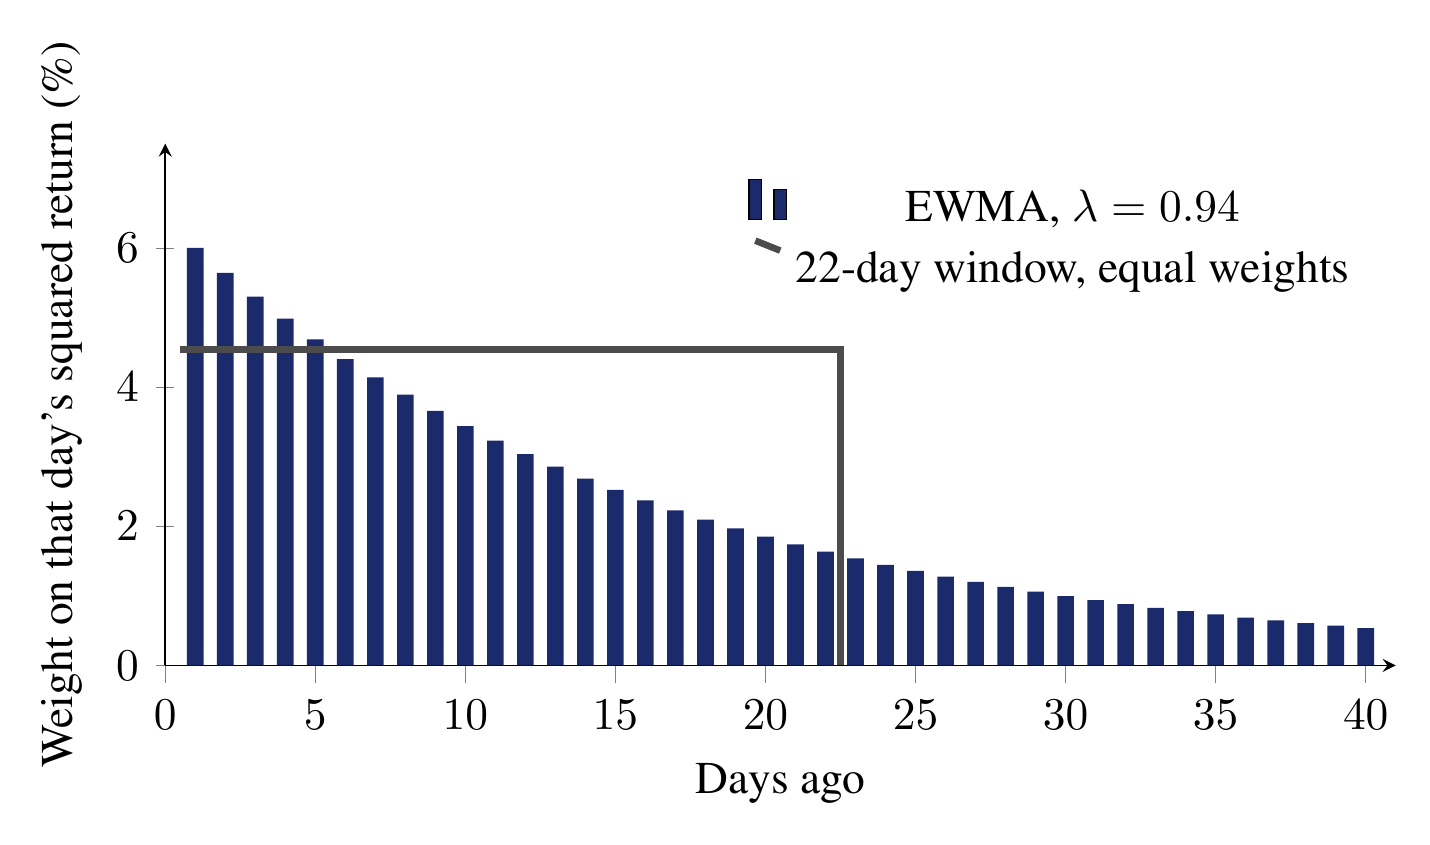
\includegraphics[width=0.85\linewidth]{images/fig11-1-ewma-weights.png}
\caption{Weights on past squared returns. A 22-day historical window gives each day the same weight and then drops it abruptly. EWMA gives the most weight to yesterday and fades older days gradually, so it reacts faster to news and never drops a day all at once.}
\label{fig:11-ewma}
\end{figure}

\textbf{GARCH(1,1)} (generalized autoregressive conditional heteroskedasticity) adds a pull toward a long-run level:
\begin{equation}
  \sigma^2_t = \omega + \alpha\,r^2_{t-1} + \beta\,\sigma^2_{t-1}
  \label{eq:11-garch}
\end{equation}
Here $\alpha$ measures how strongly a new shock moves the forecast, and $\beta$ measures how long the effect lasts. Four quantities follow from the parameters:

\begin{itemize}
  \item \textbf{Persistence} is $\alpha + \beta$, which must be below 1.
  \item The \textbf{long-run variance} is $V = \omega / (1 - \alpha - \beta)$.
  \item Forecasts revert to $V$ geometrically: the expected variance $k$ days ahead is
  \begin{equation}
    E_t[\sigma^2_{t+k}] = V + (\alpha + \beta)^{k-1}\left(\sigma^2_{t+1} - V\right)
    \label{eq:11-forecast}
  \end{equation}
  \item The \textbf{half-life} of a volatility shock, the time for half of it to fade, is $\ln 0.5 / \ln(\alpha + \beta)$.
\end{itemize}

EWMA is the special case $\omega = 0$, $\alpha = 1 - \lambda$, $\beta = \lambda$, with persistence exactly 1, so EWMA forecasts never revert. \textbf{GJR-GARCH} adds a term $\gamma\,r^2_{t-1}\,\mathbf{1}[r_{t-1} < 0]$, where the indicator $\mathbf{1}[\cdot]$ is 1 when its condition holds and 0 otherwise, so falls raise volatility more than rises. This asymmetry is the \textbf{leverage effect}. The parameters are estimated by \textbf{maximum likelihood}: choosing the values that make the observed returns most probable under the model.

\textbf{Realized variance} sums squared returns within a period, such as squared five-minute returns within a day. With enough intraday data it measures that day's variance almost exactly. The \textbf{HAR model} (heterogeneous autoregressive) forecasts tomorrow's realized variance by regressing it on the averages of the last day, week and month.

\textbf{Implied volatility} is the volatility that makes an option's market price equal its model price (Chapter 14). The \textbf{VIX} is the market's 30-day implied volatility for the S\&P 500, computed from a strip of index options. It is a forecast under the \emph{risk-neutral} measure, the probabilities that price assets as if investors did not care about risk, not the real-world probabilities. Investors pay a premium to insure against volatility, so the VIX usually exceeds the volatility that follows. The gap is the \textbf{variance risk premium}.

\textbf{Worked example.} Yesterday's daily volatility estimate was 1.6\% (variance 0.000256), and the market then fell 3\% ($r^2 = 0.0009$).

\begin{itemize}
  \item EWMA with $\lambda = 0.94$: $\sigma^2 = 0.94 \times 0.000256 + 0.06 \times 0.0009 = 0.000295$. Volatility rises to 1.72\% a day, or 27\% annualized.
  \item GARCH with $\omega = 0.000002$, $\alpha = 0.08$ and $\beta = 0.90$:
  \begin{itemize}
    \item $\sigma^2 = 0.000002 + 0.08 \times 0.0009 + 0.90 \times 0.000256 = 0.000304$, or 1.74\% a day.
    \item Persistence is 0.98, so the long-run variance is $0.000002 / 0.02 = 0.0001$: 1\% a day, or 15.9\% a year. The half-life is $\ln 0.5 / \ln 0.98 \approx 34$ trading days (Figure~\ref{fig:11-garch}).
    \item The variance over the next ten days is $10 \times 0.0001 + (0.000304 - 0.0001) \times (1 - 0.98^{10})/(1 - 0.98) = 0.00287$. Ten-day volatility is 5.4\%, or 26.9\% annualized. That is below the 27.7\% you would get by assuming today's 1.74\% persists, because the forecast is already reverting.
  \end{itemize}
\end{itemize}

\begin{figure}[htbp]
\centering
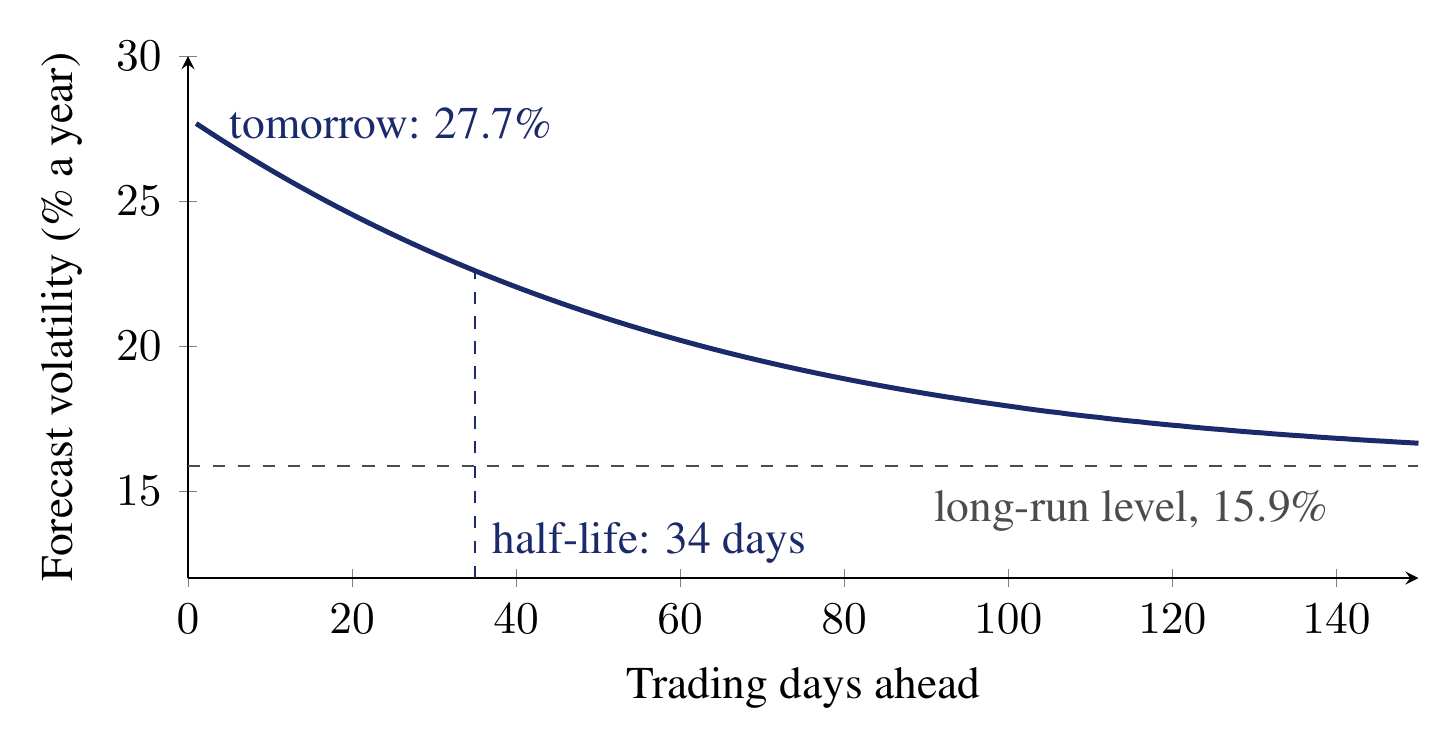
\includegraphics[width=0.85\linewidth]{images/fig11-2-garch-reversion.png}
\caption{A GARCH forecast reverting to its long-run level, from the worked example. After a 3\% fall the forecast for tomorrow is 27.7\% a year; it then decays toward 15.9\%, losing half of the gap every 34 trading days.}
\label{fig:11-garch}
\end{figure}

\textbf{Further reading.} Hull, \emph{Options, Futures, and Other Derivatives} (chapter on estimating volatilities and correlations: EWMA, GARCH, maximum likelihood) and \emph{Risk Management and Financial Institutions}; Tsay, \emph{Analysis of Financial Time Series} (conditional heteroskedastic models); Campbell, Lo and MacKinlay, \emph{The Econometrics of Financial Markets}; Taylor, \emph{Asset Price Dynamics, Volatility, and Prediction}; Poon, \emph{A Practical Guide to Forecasting Financial Market Volatility}.

\section{How it works}
\label{sec:11-how}

Three regularities in daily stock returns, all documented in Chapter 3 (Section~\ref{sec:03-facts}), motivate every model in this chapter.

\begin{itemize}
  \item \textbf{Volatility clustering.} Mandelbrot (1963) observed that large changes tend to be followed by large changes, of either sign, and small changes by small changes. Returns themselves have almost no autocorrelation, but absolute and squared returns are positively autocorrelated, and the autocorrelation decays slowly over weeks and months. A forecastable size combined with an unforecastable sign is exactly what an efficient market with changing risk would produce.
  \item \textbf{Fat tails.} Daily returns have far more extreme days than a normal distribution allows. Part of this is clustering itself: a mixture of calm and turbulent periods, each roughly normal, has fat tails overall. Even after allowing for clustering, the standardized returns $r_t / \sigma_t$ remain somewhat fat-tailed, which is why many applications use Student-$t$ shocks.
  \item \textbf{The leverage effect.} Volatility rises more after falls than after rises of the same size. Black (1976) attributed this to leverage, since a falling share price raises a firm's debt-to-equity ratio and so the riskiness of its equity. The effect is too large to be explained by leverage alone, and it is strongest for the index. Risk premiums and \textbf{volatility feedback}, in which higher expected volatility lowers prices, both contribute.
\end{itemize}

The models differ in how they turn past returns into a forecast.

\begin{itemize}
  \item \textbf{Historical and EWMA} forecasts are smoothing rules with one choice: the window length or $\lambda$.
  \item \textbf{GARCH} models are estimated, have a long-run level and revert toward it. At long horizons their forecasts converge to the \textbf{unconditional variance}, the long-run average, which is right if volatility truly mean-reverts and costly if the long-run level itself shifts.
  \item \textbf{HAR} captures the slow decay of volatility's memory with three regressors, one per horizon. It is linear and estimated by ordinary least squares, which makes it easy to extend.
  \item \textbf{The VIX} is not a model of past returns. It is a market price that can embed information about scheduled events, such as elections and central bank meetings, that no time-series model sees. It also embeds the variance risk premium, so it is biased upward as a forecast.
\end{itemize}

Figure 11.4, from the lab, shows the pattern the models exploit. On U.S. data the bars for returns hover near zero at every lag. The bars for absolute returns are positive at lag 1 and still clearly positive after 50 trading days.

\section{The claim}
\label{sec:11-claim}

\begin{callout}
\textbf{Claim.} Today's volatility forecasts tomorrow's. Forecasts built from past returns, or from option prices, beat a constant forecast by a wide margin, out of sample, at horizons from one day to one month.
\end{callout}

To test the claim we need to be precise on four points.

\begin{itemize}
  \item \textbf{What is forecast.} The target is the variance of the market's return over the next $h$ days, for $h = 1$, 5 and 22. True variance is never observed, so we use a \textbf{proxy}, an observable stand-in: the sum of squared daily returns over those days.
  \item \textbf{Against what.} The weakest benchmark is the \textbf{long-run average}, a constant. Beating it shows that volatility is forecastable at all. The stronger benchmark is a \textbf{random walk} in volatility: last month's variance continues. Beating that shows that a model adds something beyond the obvious.
  \item \textbf{How it is scored.} We use two loss functions, MSE and QLIKE, explained in Section~\ref{sec:11-eval}. The choice matters more than it does for return forecasts.
  \item \textbf{What would count against it.} The claim fails if forecasts beat the long-run average only in sample, or only in calm periods. It weakens if the gain disappears at horizons beyond a few days, or if no model beats the random walk.
\end{itemize}

A second, separate claim concerns use: that an investor who holds less of the market when forecast volatility is high earns a higher Sharpe ratio. Forecastable volatility is necessary for that claim but not sufficient. Expected returns may rise with volatility, and trading has costs.

\section{The original evidence}
\label{sec:11-evidence}

\textbf{ARCH and GARCH.} Engle (1982) introduced the ARCH model, in which today's variance depends on past squared shocks. His first application was to U.K. inflation, not stock returns. Bollerslev (1986) added lagged variance, producing GARCH(1,1), which captures long memory with three parameters. Within a decade GARCH-type models had been fitted to almost every financial series, with the same finding each time: persistence close to 1, so volatility shocks die out over weeks to months. Glosten, Jagannathan and Runkle (1993) added the asymmetric term that bears their initials and found strong leverage effects in U.S. stock returns. Engle shared the 2003 Nobel prize for this work.

\textbf{The low-$R^2$ puzzle and its resolution.} Early out-of-sample tests seemed discouraging. Regressions of daily squared returns on GARCH forecasts gave $R^2$ of only a few percent, and some authors concluded that GARCH forecasts were poor. Andersen and Bollerslev (1998) showed that the problem was the target, not the forecast. A single squared return is an extremely noisy measure of that day's variance, so even a perfect forecast must have a low $R^2$ against it. Measured against realized variance from intraday returns, the same GARCH forecasts explained around half of the variation.

\textbf{Realized volatility and HAR.} Andersen, Bollerslev, Diebold and Labys (2003) treated realized variance as an observable series and modelled it directly. Simple time-series models of realized variance outperformed GARCH models estimated on daily returns. Corsi (2009) proposed the HAR model, motivated by traders who operate at daily, weekly and monthly horizons. It reproduces volatility's long memory with three regressors and has become the standard benchmark for realized-variance forecasts.

\textbf{Horse races.} Hansen and Lunde (2005) compared 330 models on a Deutsche mark--dollar exchange rate and IBM stock returns. For the exchange rate, nothing significantly beat GARCH(1,1). For IBM, GARCH(1,1) was clearly inferior to models with a leverage effect. Poon and Granger (2003) reviewed 93 studies. Implied volatility generally forecast best, followed by historical volatility and GARCH roughly together, and all methods did better than a constant.

\section{Evaluating volatility forecasts}
\label{sec:11-eval}

Scoring a volatility forecast is harder than scoring a return forecast, because the thing being forecast is never observed. Every comparison uses a proxy, such as the sum of squared daily returns. The proxy is unbiased but noisy. The question is whether the noise can change which model wins.

Patton (2011) answered it. With a noisy proxy, only some loss functions are \textbf{robust}: they rank forecasts in the same order as they would against the true variance. Two common ones are robust (Figure~\ref{fig:11-qlike}).

\begin{itemize}
  \item \textbf{MSE}, $(RV - F)^2$, where $RV$ is the proxy and $F$ the forecast. It is robust but dominated by the largest days. A few crisis days can decide the whole comparison.
  \item \textbf{QLIKE}, $\log F + RV/F$, the loss implied by the normal likelihood. It is robust and penalizes forecasts that are too \emph{low} much more than forecasts that are too high, which suits risk management. Because it depends on the ratio $RV/F$, it is not dominated by the level of volatility in crises.
\end{itemize}

\begin{figure}[htbp]
\centering
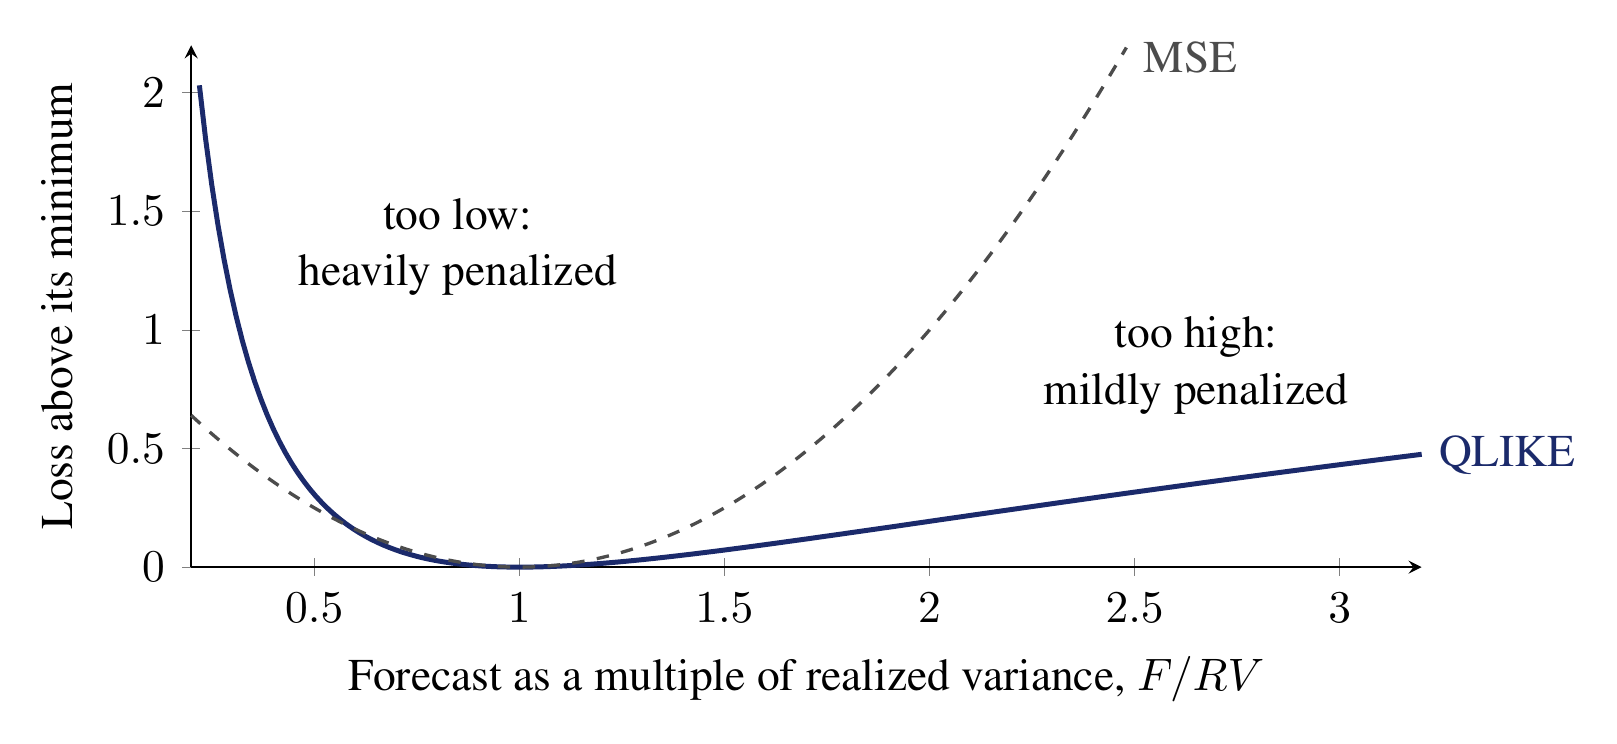
\includegraphics[width=0.85\linewidth]{images/fig11-3-qlike.png}
\caption{Two robust loss functions, measured from their minimum. MSE treats a forecast that is too high and one that is too low symmetrically. QLIKE punishes a forecast that is too low far more than one that is too high: underestimating risk is the costlier mistake.}
\label{fig:11-qlike}
\end{figure}

Others are not robust. Mean absolute error and MSE on volatility rather than variance, both common in early studies, can rank a biased forecast above the true variance when the proxy is noisy. They should be avoided.

Two diagnostics complement the loss comparison.

\begin{itemize}
  \item \textbf{Mincer--Zarnowitz regression.} Regress realized on forecast variance. An unbiased forecast has intercept 0 and slope 1. A slope below 1 means the forecast overreacts, which is typical of the VIX because of the variance risk premium. The $R^2$ measures informativeness but is capped by the noise in the proxy, as Andersen and Bollerslev showed.
  \item \textbf{Diebold--Mariano test} (Chapter 5). Test whether the average loss difference between two models is zero, using Newey--West errors with $h - 1$ lags, since multi-day targets overlap.
\end{itemize}

A fair comparison also requires real-time forecasts. Every parameter must be estimated only on data available at the forecast date, as in the walk-forward design of Chapter 5.

\section{Replication lab: forecasting market volatility}
\label{sec:11-lab}

\begin{callout}
\textbf{Lab 11 at a glance.} \emph{Claim on trial:} volatility is predictable. \emph{Data:} U.S. market returns since 1926, from the daily factors in the Kenneth French library, and, from 1990, the VIX from FRED; both are free. \emph{Code:} runs as a script (\texttt{python lab11.py}) or as a notebook with a prediction prompt before each step.
\end{callout}

\textbf{Part A, stylized facts.} It computes autocorrelations of daily returns and absolute returns at lags 1 to 50, and the correlation between today's return and tomorrow's absolute return (Figure 11.4). Expect the first to hover near zero, the second to stay positive for months, and the third to be negative: the leverage effect.

\textbf{Part B, forecast comparison.} Each trading day from 1990, the lab forecasts the market's variance over the next 1, 5 and 22 days with seven methods:

\begin{center}
\small
\begin{tabularx}{0.9\linewidth}{@{}>{\raggedright\arraybackslash}p{0.20\linewidth}>{\raggedright\arraybackslash}X>{\raggedright\arraybackslash}p{0.33\linewidth}@{}}
\toprule
Method & Forecast & Parameters \\
\midrule
Long-run average & Mean squared return to date & None \\
Random walk & Last 22 days' variance continues & None \\
EWMA & RiskMetrics, $\lambda = 0.94$ & Fixed \\
GARCH(1,1) & Mean-reverting, normal likelihood & Re-estimated yearly on the past 20 years \\
GJR-GARCH & GARCH with the leverage term & Re-estimated yearly \\
HAR & Regression on 1-, 5- and 22-day averages & Re-estimated yearly by OLS \\
VIX & $(\mathrm{VIX}/100)^2 \times h/252$ & None \\
\bottomrule
\end{tabularx}
\end{center}

Each method is scored against the random walk with QLIKE and MSE, with Diebold--Mariano tests and Mincer--Zarnowitz regressions. Figure 11.5 plots one-month forecasts through 2007--2010 against the volatility that followed. Figure 11.6 ranks the methods at each horizon.

\textbf{Part C, crises.} The same losses are computed within 2008--09, 2020 and 2022 (Figure 11.7).

\textbf{Part D, use.} A \textbf{volatility-managed portfolio} holds the market with weight proportional to 1 / last month's realized variance, scaled so its volatility matches the market's, as in Moreira and Muir (2017). The lab reports Sharpe ratio, drawdown and alpha against the market, net of a cost per unit of weight change, with an optional leverage cap (Figure 11.8).

Three design choices affect the results. First, the proxy is built from daily returns, because intraday data are not freely available back to 1926. That makes every model look worse than in studies using five-minute data, but it does not bias the ranking under QLIKE. Second, the HAR model here uses squared daily returns, a much noisier input than the realized variance Corsi used, so expect it to do less well than in the literature. Third, the VIX was redefined in 2003; FRED's VIXCLS uses the current method throughout.

\textbf{What the simulated run shows.} On simulated GJR-GARCH data, the lab recovers what it should. Every dynamic model beats the long-run average by a wide margin. GJR, the true model, ranks first under QLIKE at all three horizons. The simulated VIX shows the upward bias built into it. These results confirm that the code works. They say nothing about real markets. Run the lab on the real data to reach your own verdict.

\section{Stress tests}
\label{sec:11-stress}

\textbf{Horizon.} Forecastability is a short-horizon phenomenon. Because GARCH persistence is below 1, every GARCH forecast converges to the long-run level. Beyond a few months, a constant forecast is hard to beat, and over years, estimates of the long-run level itself drift. At one day to one month, the horizons in the lab, the evidence for forecastability is strong in the literature. The lab lets you measure how fast the advantage over the long-run average shrinks.

\textbf{Crises.} Volatility jumps faster than any model built on past returns can follow. In the first days of October 2008 and of March 2020, every time-series forecast was far too low. QLIKE punishes exactly that error. The models catch up within days, and because they then revert too slowly, they overpredict as the crisis fades. The VIX, as a market price, can react within the day to news and is the obvious candidate to do better at the onset. Figure 11.7 tests whether it did.

\textbf{The 2022 rate shock.} In 2022 stocks fell by about a fifth, but realized volatility stayed moderate, without a single spike. This is a useful contrast with 2008 and 2020. A model that forecasts volatility well can still miss a large, slow decline, because volatility and losses are different things.

\textbf{Estimation window.} GARCH parameters estimated on 20 years that include 2008 differ from those estimated on calmer windows. Persistence near 1 means that small changes in $\alpha + \beta$ produce large changes in long-horizon forecasts. Rerun Part B with \texttt{-{}-window-years 10} and compare.

\textbf{Proxy.} A sum of squared daily returns is noisy, especially at the 1-day horizon, where it is a single squared return. Andersen and Bollerslev (1998) showed that this lowers every model's $R^2$ but, with a robust loss, does not change the ranking. Liu, Patton and Sheppard (2015) compared nearly 400 realized-variance estimators and found that five-minute realized variance is hard to beat. Students with intraday data can replace the proxy and check.

\section{Verdict}
\label{sec:11-verdict}

\begin{callout}
\textbf{Verdict: survives, strongly, at horizons from one day to one month} (as of October 2026). The claim about \emph{using} volatility forecasts to improve a market investor's Sharpe ratio is a separate one, and it \textbf{weakens} once forecasts are made in real time and costs and leverage limits are applied.
\end{callout}

The case for the forecasting claim rests on four findings.

\begin{itemize}
  \item \textbf{It replicates across markets, assets and decades.} Volatility clustering appears in every liquid market studied, back to the nineteenth century. GARCH-type models fitted to them give persistence close to 1.
  \item \textbf{It holds out of sample.} In real-time forecasts, dynamic models beat the long-run average by a wide margin. That is the result Lab 11 is built to check on U.S. data since 1990.
  \item \textbf{It survives the right loss functions.} Early doubts came from evaluating against a noisy proxy with an unsuitable loss. Andersen and Bollerslev (1998) and Patton (2011) removed both problems.
  \item \textbf{It has a plausible mechanism.} News arrives in clusters, and uncertainty is persistent. Nothing about forecastable volatility contradicts market efficiency, since it predicts risk, not returns.
\end{itemize}

The qualifications are about \emph{how much}, not \emph{whether}.

\begin{itemize}
  \item \textbf{Complex models add little over simple ones.} EWMA and GARCH(1,1) are hard to beat for many series. A leverage term helps for equity indices. HAR helps most when realized variance from intraday data is available.
  \item \textbf{The advantage fades with horizon.} Beyond a few months, forecasts converge to a long-run level that is itself uncertain.
  \item \textbf{Every model is late at the onset of a crisis.} Forecasts built from past returns cannot anticipate the first violent day. They are most useful after it.
  \item \textbf{The VIX is informative but biased.} It contains the variance risk premium, so it overstates future volatility on average. It must be adjusted before it is used as a forecast.
\end{itemize}

\section{What investors can use}
\label{sec:11-investors}

\textbf{Risk forecasts, yes.} Any investor sizing positions, setting stop-losses or computing margin should use a volatility forecast that reacts to recent data, such as EWMA or GARCH, rather than a long-run average. This is uncontroversial and is the basis of Value at Risk (Chapter 13).

\textbf{Volatility timing for returns: be skeptical.} Moreira and Muir (2017) found that scaling exposure to the market inversely to last month's variance produced an alpha of about 4.9\% a year over 1926--2015, with similar results for several factors. \textbf{Volatility-targeting} funds and \textbf{risk-parity} strategies, which allocate so that each asset contributes equal risk, apply versions of the idea. Three later findings temper it.

\begin{itemize}
  \item \textbf{Real-time feasibility.} Cederburg, O'Doherty, Wang and Yan (2020) tested 103 equity strategies. The alphas in \textbf{spanning regressions}, regressions of the managed portfolio on the original, were real, but exploiting them required combining the managed and unmanaged portfolios with weights estimated in sample. Implemented out of sample, the managed versions generally did no better than the originals, because the spanning regressions were unstable.
  \item \textbf{Leverage.} The managed portfolio's weight on the market often exceeds 1 in calm periods. In the lab's simulated run it averaged 1.4 and peaked near 10. Capping leverage at a realistic level reduces the gains.
  \item \textbf{Costs and crowding.} Turnover is high when volatility changes quickly, and volatility-targeting funds all sell at the same time, which can deepen the declines they are trying to avoid.
\end{itemize}

The benefit is clearer for momentum, where crashes follow high volatility (Barroso and Santa-Clara 2015; Chapter 9), than for the market.

\textbf{Questions to ask a manager who uses volatility targeting:}

\begin{itemize}
  \item What volatility forecast do you use, and how quickly does it react?
  \item What is the maximum leverage, and what happens to turnover in a volatility spike?
  \item Is the backtest scaled using information available at the time, or using full-sample volatility?
  \item How did the strategy perform in February 2018 and March 2020, when volatility jumped within days?
\end{itemize}

\begin{callout}
\textbf{What Failed: selling volatility before February 5, 2018.} For years before 2018, products that bet against volatility were among the best performers in the market. The VelocityShares Daily Inverse VIX Short-Term ETN (XIV) earned the variance risk premium by shorting VIX futures, and it held \$1.9 billion in assets. On February 5, 2018, the VIX rose 115.6\%, its largest one-day increase ever. XIV lost 96.3\% of its value that day, and Credit Suisse, its issuer, closed it within weeks.

The episode does not contradict this chapter. Volatility forecasts are informative on average. But a forecast that volatility will stay low is weakest exactly when it matters most: at the onset of a spike. A strategy that earns a small premium most days and loses almost everything on one day can look excellent in any backtest that misses that day. Chapter 13 returns to this problem.
\end{callout}

\section{Open questions}
\label{sec:11-open}

\begin{itemize}
  \item \textbf{Does volatility timing pay after costs?} The evidence for the market is mixed. Does it hold for factors such as momentum, and in other countries?
  \item \textbf{What is the right long-run level?} GARCH forecasts revert to a constant, but the evidence suggests slow-moving changes in average volatility, linked to the business cycle and macroeconomic uncertainty. Component GARCH and GARCH-MIDAS models try to capture this. Do they forecast better at long horizons?
  \item \textbf{Can machine learning beat HAR?} Recent studies add many predictors, such as news, macroeconomic data and other assets' volatilities. Do the gains survive the out-of-sample discipline of Chapters 4 and 5?
  \item \textbf{What does the VIX know?} Implied volatility combines a forecast with a risk premium. Can the two be separated well enough to improve the forecast?
\end{itemize}

\section*{Exercises}
\addcontentsline{toc}{section}{Exercises}

\subsection*{Conceptual (all readers)}

\begin{enumerate}
  \item A GARCH(1,1) model has $\omega = 0.000003$, $\alpha = 0.10$ and $\beta = 0.88$. (a) What are the long-run daily and annualized volatilities? (b) What is the half-life of a shock? (c) If tomorrow's variance forecast is 0.0004, what is the forecast volatility over the next 22 days, annualized?
  \item Show that EWMA is GARCH(1,1) with $\omega = 0$. What does this imply for EWMA forecasts at long horizons?
  \item A colleague argues that because volatility is forecastable, markets cannot be efficient. Explain why forecastable volatility is consistent with efficiency, and what evidence would change your answer.
\end{enumerate}

\subsection*{Lab extensions (technical readers)}

\begin{enumerate}
  \setcounter{enumi}{3}
  \item Part A: compute the autocorrelations of squared returns as well as absolute returns. Which decays faster, and why might extreme days explain the difference?
  \item Part B: rank the models by MSE instead of QLIKE. Does the ranking change? Which days drive the MSE comparison?
  \item Part B: estimate GARCH with Student-$t$ shocks, using the option \texttt{dist="t"} of \texttt{fit\_garch}. Does it forecast better than the normal version?
  \item Part B: regress realized variance on both the GJR forecast and the VIX. Does each add information? Compare the VIX's Mincer--Zarnowitz slope with 1 and explain.
  \item Part C: for the first ten trading days of October 2008 and of March 2020, plot each forecast against realized variance. How many days did each model take to catch up?
  \item Part D: rescale the managed portfolio using only past data and cap the weight at 1.5. How much of the alpha survives? Compare with Cederburg et al.\ (2020).
\end{enumerate}

\section*{References}
\addcontentsline{toc}{section}{References}

\begin{itemize}
  \item Andersen, T. G. and Bollerslev, T. (1998). Answering the Skeptics: Yes, Standard Volatility Models Do Provide Accurate Forecasts. \emph{International Economic Review} 39(4): 885--905.
  \item Andersen, T. G., Bollerslev, T., Diebold, F. X. and Labys, P. (2003). Modeling and Forecasting Realized Volatility. \emph{Econometrica} 71(2): 579--625.
  \item Barroso, P. and Santa-Clara, P. (2015). Momentum Has Its Moments. \emph{Journal of Financial Economics} 116(1): 111--120.
  \item Black, F. (1976). Studies of Stock Price Volatility Changes. \emph{Proceedings of the 1976 Meetings of the American Statistical Association, Business and Economic Statistics Section}: 177--181.
  \item Bollerslev, T. (1986). Generalized Autoregressive Conditional Heteroskedasticity. \emph{Journal of Econometrics} 31(3): 307--327.
  \item Cederburg, S., O'Doherty, M. S., Wang, F. and Yan, X. (2020). On the Performance of Volatility-Managed Portfolios. \emph{Journal of Financial Economics} 138(1): 95--117.
  \item Corsi, F. (2009). A Simple Approximate Long-Memory Model of Realized Volatility. \emph{Journal of Financial Econometrics} 7(2): 174--196.
  \item Engle, R. F. (1982). Autoregressive Conditional Heteroscedasticity with Estimates of the Variance of United Kingdom Inflation. \emph{Econometrica} 50(4): 987--1007.
  \item Glosten, L. R., Jagannathan, R. and Runkle, D. E. (1993). On the Relation between the Expected Value and the Volatility of the Nominal Excess Return on Stocks. \emph{Journal of Finance} 48(5): 1779--1801.
  \item Hansen, P. R. and Lunde, A. (2005). A Forecast Comparison of Volatility Models: Does Anything Beat a GARCH(1,1)? \emph{Journal of Applied Econometrics} 20(7): 873--889.
  \item J.P. Morgan/Reuters (1996). \emph{RiskMetrics---Technical Document} (4th ed.). New York: Morgan Guaranty Trust Company.
  \item Liu, L. Y., Patton, A. J. and Sheppard, K. (2015). Does Anything Beat 5-Minute RV? A Comparison of Realized Measures across Multiple Asset Classes. \emph{Journal of Econometrics} 187(1): 293--311.
  \item Mandelbrot, B. (1963). The Variation of Certain Speculative Prices. \emph{Journal of Business} 36(4): 394--419.
  \item Moreira, A. and Muir, T. (2017). Volatility-Managed Portfolios. \emph{Journal of Finance} 72(4): 1611--1644.
  \item Patton, A. J. (2011). Volatility Forecast Comparison Using Imperfect Volatility Proxies. \emph{Journal of Econometrics} 160(1): 246--256.
  \item Poon, S.-H. and Granger, C. W. J. (2003). Forecasting Volatility in Financial Markets: A Review. \emph{Journal of Economic Literature} 41(2): 478--539.
\end{itemize}

\textbf{Data:} Kenneth R. French Data Library, Fama/French 3 Factors [Daily]. Chicago Board Options Exchange, CBOE Volatility Index: VIX [VIXCLS], retrieved from FRED, Federal Reserve Bank of St.\ Louis.
